%Einfache Vorlage f�r eine mit Latex realisierte Hausarbeit von http://www.studieren-info.de
%Du kannst diese Vorlage f�r deine Hausarbeit beliebig anpassen%


%-------------------
%Beginn des Kopfbereiches
%-------------------

%Wir verwenden eine DIN-A4-Seite und die Schriftgr��e 12.
\documentclass[a4paper,12pt,fontsize=12,DIV=12]{scrartcl} 


%Diese drei Pakete ben�tigen wir f�r die Umlaute, Deutsche Silbentrennung etc.
%Apple-Nutzer sollten anstelle von \usepackage[latin1]{inputenc} das Paket \usepackage[applemac]{inputenc} verwenden
\usepackage[utf8]{inputenc}
\usepackage[ngerman]{babel}
\usepackage[T1]{fontenc}
\usepackage{graphicx}
\usepackage{subfigure}
\usepackage[format=hang,justification=centering,singlelinecheck=off]{caption}
%\packet für die Einfügung von Quellcode
\usepackage{listings}
\usepackage{color}


%Das Paket erzeugt ein anklickbares Verzeichnis in der PDF-Datei.
\usepackage{hyperref}

%Das Paket wird für die anderthalb-zeiligen Zeilenabstand benötigt
\usepackage{setspace}

%Einrückung eines neuen Absatzes
\setlength{\parindent}{0em}

%Definition der Ränder
\usepackage[paper=a4paper,left=30mm,right=30mm,top=30mm,bottom=30mm]{geometry} 

%Abstand der Fußnoten
\deffootnote{1em}{1em}{\textsuperscript{\thefootnotemark\ }}

%Regeln, bis zu welcher Tiefe (section,subsection,subsubsection) Überschriften angezeigt werden sollen (Anzeige der Überschriften im Verzeichnis / Anzeige der Nummerierung)
\setcounter{tocdepth}{3}
\setcounter{secnumdepth}{3}

\addtokomafont{disposition}{\color{blue}}
%alle Überschriften und Sectionziffern einfärben

%\pagecolor{cyan}
%Seitenhintergrundfarbe bestimmen

%-------------------
%Ende des Kopfbereiches
%-------------------


%-------------------
%Hier beginnt der Text deiner Hausarbeit
%-------------------
\begin{document}


%Beginn der Titelseite
\begin{titlepage}
\begin{small}
\vfill {Universitaet Rostock\\ 
IEF/Institut für Automatisierungstechnik\\ 
Sommersemester 2012}
\end{small}


\begin{center}
\begin{Large}
\vfill {\textsf{\textbf{
	\textcolor{blue}{Hausarbeit - Hall-Software für das EZ-Kit BF533}
}}}
\end{Large}
\end{center}

\begin{center}
\vspace{2.0cm}
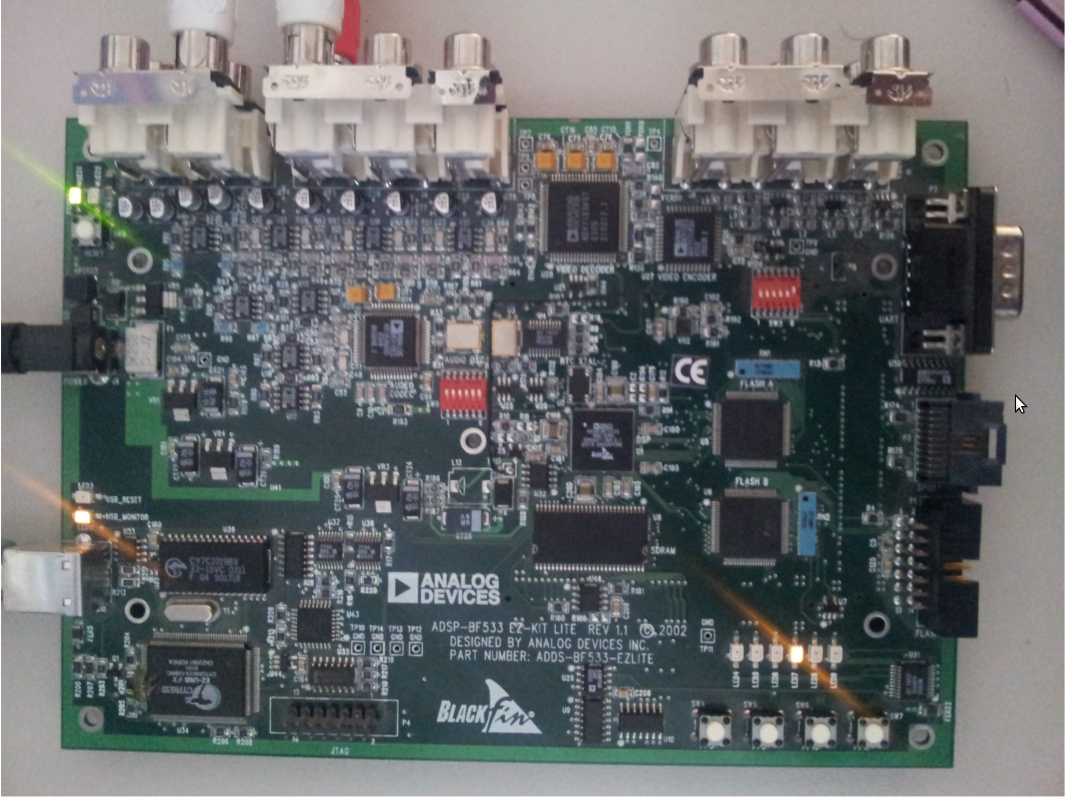
\includegraphics[scale=0.1]{Bilder/Signalprozessor.jpg}
\end{center}

\begin{small}
\vfill Florian Grützmacher \\ Max-Planck-Str. 2a \\  18057 Rostock \\  florian.gruetzmacher@uni-rostock.de\\ 
\end{small}

\vspace{-1.0cm}

\begin{small}
\vfill Simeon Wiedenmann \\ Kiebitzberg 4 \\  18057 Rostock \\  simeon.wiedenmann@uni-rostock.de\\ 
\newline
\today
\end{small}

\end{titlepage}
%Ende der Titelseite


%Inhaltsverzeichnis (aktualisiert sich erst nach dem zweiten Setzen)
\tableofcontents
\thispagestyle{empty}

%Beginn einer neuen Seite
\clearpage

%Anderthalbzeiliger Zeilenabstand ab hier
\onehalfspacing

\pagestyle{plain}


\section{Einleitung}
Im Rahmen der Veranstaltungsreihe "`Signalprozessortechnik"' am Institut für Automatisierungstechnik der Universität Rostock wurden Kenntnisse über Funktionen und Leistungsfähigkeit verschiedener Signalprozessoren für den Einsatz digitaler Signalverarbeitung vermittelt.\footnote{siehe Vorlesungsverzeichnis der Universität Rostock, Veranstaltungsnr. 24141 }
Die Veranstaltung wurde im Sommersemester 2012 durch die Fakultät für Informatik und Elektrotechnik (IEF) der Universität Rostock angeboten und von Herrn Dr.-Ing. Wolf-Dieter Heinitz gehalten.
Neben den behandelten Schwerpunkten

 %Eine einfache Liste
 \begin{itemize} 
\item Digitale Signalverarbeitung: Vorteile, Probleme, Applikationen
\item Basisalgorithmen der digitalen Signalverarbeitung
\item Datenformate für die digitale Signalverarbeitung
\item Signalverarbeitung mit klassischen Mikrokontrollern
\item Universelle Signalprozessoren: Festkomma-Prozessor DSP 5630x, Gleitkomma-Prozessor TMS 320C3x, TMS320C4x
\item Übersicht zu anderen modernen Signalprozessoren und aktuellen Weiterentwicklungen Texas Instruments: C80, C62x, C67x, Analoge Devices: ADSP-21160, BF53x
\item Entwicklungswerkzeuge für DSP-Programmierung
\end{itemize}

galt es ein Abschlussprojekt zu Implementieren, es den Modulteilnehmern vorzustellen und das Vorgehen in einer Hausarbeit zu dokumentieren.

\section{Aufgabenstellung}

\subsection{Hall-Software für das EZ-Kit BF533}
Programmierung einer Software zur Erzeugung von künstlichem Hall. Ein analoges Eingangssignal von einem Mikrophon ist mit künstlichem Hall zu versehen und an einem analogen Ausgangskanal an einen Kopfhörer auszugeben.
\newline
Die Projektarbeit ist im Rahmen einer Demonstration an einem Testaufbau mit Mikrophon und Kopfhörer vorzuführen.

\subsection{Versuchsaufbau}
Bei der Implementation des künstlichen Halls ist es hilfreich, zunächst das Übertragungsverhalten des Digitalen Signalprozessors (DSP) beobachten zu können. Dazu wurde ein Versuchsaufbau für die Implementation eingerichtet, welcher hier zu sehen ist:
\begin{center}
%\vspace{2.0cm}
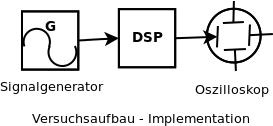
\includegraphics[scale=0.8]{Bilder/Versuchsaufbau_Implementation.png}
\end{center}
Ein am Signalgenerator erzeugtes Wunsch-Signal kann hierbei im DSP bearbeitet werden und das modifizierte Signal kann am Oszilloskop beobachtet werden.

Zur Demonstration des mit dem DSP erzeugten künstlichen Halls wird für bessere Anschaulichkeit jedoch folgender Versuchsaufbau genutzt.
\begin{center}
	%\vspace{2.0cm}
	
\includegraphics[scale=0.8]{Bilder/Versuchsaufbau_Demonstration.png}
\end{center}
%
%\begin{figure}
%	
\includegraphics[scale=0.8]{Bilder/Versuchsaufbau_Demonstration.png}
%	\caption{Titel der Grafik}
%	\label{labelname}
%\end{figure}
%
Ein Mikrofon wird an den Eingang des DSP angeschlossen und liefert ein analoges Eingangssignal. Dieses wird mit Hilfe eines Analog-Digital-Wandlers (ADC) digitalisisert und im DSP bearbeitet. Das digital bearbeitete Signal wird über einen Digital-Analog-Wandler DAC in ein analoges Ausgangssignal gewandelt, welches an den Lautsprechern ausgegeben wird.


\section{Digitale Signalverarbeitung}
Die Digitale Signalverarbeitung als Teilgebiet der Nachrichtentechnik beschäftigt sich mit der Verarbeitung digitaler Signale unter Einsatz von digitalen Systemen, wie z.B. Digitale Signalprozessoren.
Da unsere physikalische Umwelt jedoch häufig Analoge Signale als Eingangssignale (wie z.B. das Schwingen einer Membran im Mikrofon) sowie analoge Ausgangssignale (z.B. schwingende Lautsprechermembranen) verursacht, schließt die digitale Signalverarbeitung häufig auch eine Analog-Digital Wandlung des Eingangssignals und eine Digital-Analog Wandlung des Ausgangssignals mit ein.

\subsection{Das Prinzip digitaler Signalverarbeitung}
Um ein zeit-kontinuierliches und werte-kontinuierliches analoges Signal zu digitalisieren, muss es mit einer Abtastfrequenz $f_a$ abgetastet werden und auf einen quantisierten Wertebereich abgebildet werden. 
Um eine "`exakte"' Signalrekonstruktion sicherzustellen, muss das Nyquist-Shannon-Abtasttheorem eingehalten werden. Dieses besagt, dass die Abtastfrequenz $f_a$ mindestens so groß sein muss wie das doppelte der höchsten im Signal vorkommenden Frequenz $f_g$.
\begin{center}
\fbox{$f_a >= 2*f_g$} \footnote{Abtasttheorem }\\
\end{center}
Um dies sicherzustellen wird das analoge Eingangssignal x(t) mittels eines analogen Tiefpasses (TP) bandbegrenzt. Das abgetastete Signal ist bereits zeit-diskret.
%
\begin{figure}[h]
	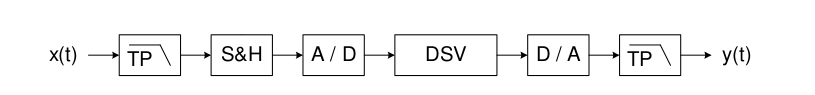
\includegraphics[scale=0.5]{Bilder/DSV_Blockschaltbild.png}
	\caption{Titel der Grafik}
	\label{labelname}
\end{figure}
%

%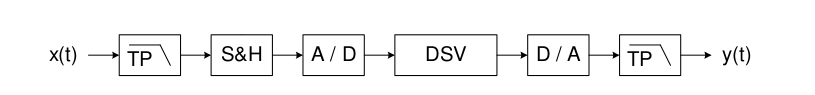
\includegraphics[scale=0.5]{Bilder/DSV_Blockschaltbild.png}


Ein Sampe and Hold Glied (S\&H) stellt sicher, dass der am Analog-Digital Wandler (A/D) anliegende Spannungswert für die Zeit eines Wandelvorgangs konstant gehalten wird.
Im Anschluss an die A/D Wandlung liegt ein zeit- und werte-diskretes Signal vor. Dieses digitale Signal kann nun mittels Digitaler Signalverarbeitung (DSV) wie gewünscht manipuliert werden. Dazu werden häuftig digitale Signalprozessoren eingesetzt.

Das digitale Signal muss nach der Verarbeitung erneut in ein analoges Signal gewandelt werden. Dies geschieht mithilfe des Digital-Analog Wandlers (D/A). Anschließend wird das Ausgangssignal noch durch einen analogen Rekonstruktions-Tiefpass (T/P) geglättet. Das so entstehende Ausgangssignal ist nun wieder analog und geht aus dem Eingangssignal x(t) durch digitale Signalverarbeitung hervor.

\subsection{Warum Signalprozessoren?}
Zzril delenit augue duis dolore te feugait nulla facilisi nam liber tempor. Nihil imperdiet doming; id quod mazim placerat facer possim assum? Mirum est notare quam littera gothica 
quam nunc putamus! Consectetuer adipiscing elit sed diam nonummy nibh euismod.

\section{Das Kit EZ-Kit BF533}
Dolore te feugait nulla facilisi nam liber tempor cum soluta nobis eleifend option. Amet consectetuer adipiscing elit sed diam nonummy nibh euismod tincidunt ut laoreet. In iis qui facit eorum; claritatem Investigationes demonstraverunt lectores legere me. In vulputate velit esse molestie consequat vel illum dolore. Wisi enim ad minim, veniam quis nostrud exerci. Facer possim assum typi non habent claritatem insitam est usus legentis lius quod.

Dolore te feugait nulla facilisi nam liber tempor cum soluta nobis eleifend option. Amet consectetuer adipiscing elit sed diam nonummy nibh euismod tincidunt ut laoreet. In iis qui facit eorum; claritatem Investigationes demonstraverunt lectores legere me. In vulputate velit esse molestie consequat vel illum dolore. Wisi enim ad minim, veniam quis nostrud exerci. Facer possim assum typi non habent claritatem insitam est usus legentis lius quod.

\section{Lösungsstrategie}
Dolore te feugait nulla facilisi nam liber tempor cum soluta nobis eleifend option. Amet consectetuer adipiscing elit sed diam nonummy nibh euismod tincidunt ut laoreet. In iis qui facit eorum; claritatem Investigationes demonstraverunt lectores legere me. In vulputate velit esse molestie consequat vel illum dolore. Wisi enim ad minim, veniam quis nostrud exerci. Facer possim assum typi non habent claritatem insitam est usus legentis lius quod.

Dolore te feugait nulla facilisi nam liber tempor cum soluta nobis eleifend option. Amet consectetuer adipiscing elit sed diam nonummy nibh euismod tincidunt ut laoreet. In iis qui facit eorum; claritatem Investigationes demonstraverunt lectores legere me. In vulputate velit esse molestie consequat vel illum dolore. Wisi enim ad minim, veniam quis nostrud exerci. Facer possim assum typi non habent claritatem insitam est usus legentis lius quod.

\subsection{Hall}
Hall bzw. Nachhall ist ein Effekt der durch kontinuierliche Reflexionen einer Schallwelle verursacht wird.
Wird eine Schallwelle an unterschiedlichen Stellen Reflektiert, und die reflektierten Wellen haben unterschiedliche Ankunftszeiten aufgrund der verschiedenen Abstände zu den reflektierenden Objekten, treffen mehrere reflektierte Schallwellen der selben Ursprungs-Schallwelle mit verschiedenen Verzögerungszeiten aufeinander. Da der Schalldruck einer Schallwelle mit zunehmender Ausbreitungszeit aufgrund Luftreibung und mit zunehmender Anzahl an Reflektionen aufgrund von Wärmeverlusten abnimmt, sind reflektierte Schallwellen umso schwächer, je weiter der Zeitpunkt ihrer Enstehung zurückliegt.
Hall wird unterteilt in frühe Reflektionen, welche 1-2 Reflektionen des Ursprungssignals sind, und diffusem Nachhall, welcher aus vielen Reflektionen mit stärkerer Abschwächung des Ursprungssignals besteht. Verantwortlich für den 'räumlichen' Klang des Halls, sind die frühen Reflektionen, wobei der Nachhall wiederum aus Reflektionen der frühen Reflektionen entsteht und für mehr 'Volumen' sorgt.


\begin{figure}[h]
	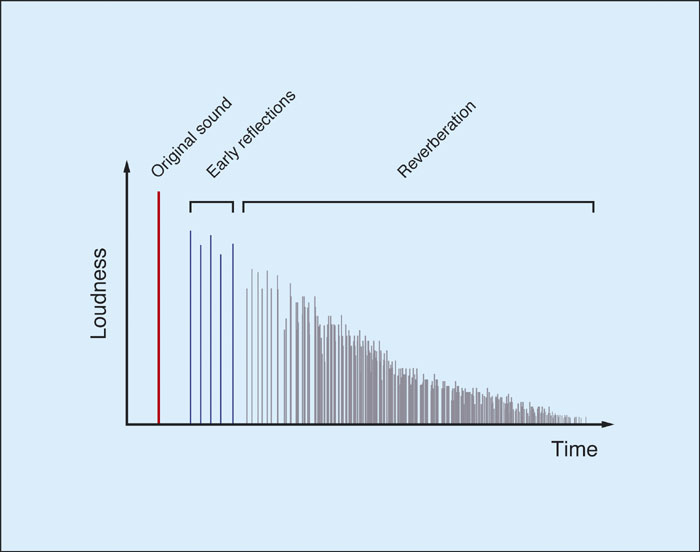
\includegraphics[scale=0.5]{Bilder/raumimpulsantwort.jpg}
	\caption{Raumimpulsantwort}
	\label{labelname}
\end{figure}
Quelle: http://www.offsetguitars.com/forums/viewtopic.php?f=11\&t=43975\&start=15

\subsection{Künstlicher Hall mit Infinite Impulse Response Filter}
Um mit dem DSP künstlichen Hall zu erzeugen, müssen die vom AD-Wandler erhaltenen Werte in einem Buffer gespeichert werden, um zu einem späteren Zeitpunkt (50 bis 100 ms) darauf zurückgreifen zu können. Jeder neu abgetastete Wert wird mit einem Vorfaktor versehen und mit weiter zurückliegenden Signalwerten, ebenfalls mit bestimmtem Vorfaktoren akkumuliert und an den DA-Wandler übergeben. Zusätlich wird der akkumulierte Wert wieder mit einem Vorfaktor auf den nächsten neuen Wert aufaddiert. Durch die Akkumulation werden die frühen Reflektionen, durch die Rückkopplung der Nachhall simuliert. 
Dies entspricht der Struktur eines IIR-Filters mit unendlicher Impulsantwort.
\begin{figure}[h]
	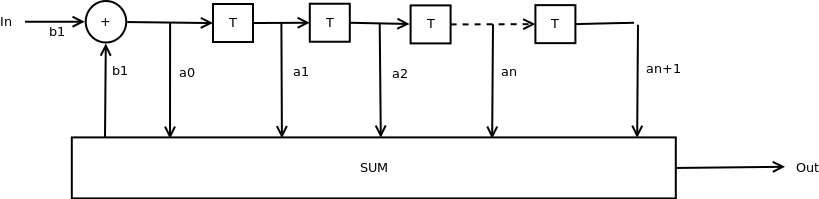
\includegraphics[scale=0.5]{Bilder/iir.png}
	\caption{IIR-Filter Struktur}
	\label{labelnameIIR-Filter Struktur}
\end{figure}

\subsection{Implementierung}
Um eine IIR-Struktur zu implementieren, haben wir einen Buffer(Array) mit 4096 Werten im fractional-32 Format deklariert. Für den Buffer und den Akkumulator wurden Fractional-32 Formate benutzt, da Multiplikationen von Fractional-16 Werten, ein Fractional-32 liefern und so ohne Schieben damit weitergerechnet werden kann.
<<<<<<< HEAD
Sobald am AD-Wandler ein neuer Wert anliegt, wird die Prozess-Funktion, im folgenden Prozess genannt, aufgerufen. Im Prozess wird der neue Wert zunächst gespeichert und mit einem dem Vorfaktor 0.5 im Buffer abgelegt. der Vorfaktor wird durch ein Right-Shift realisiert, was einer Division durch 2 entspricht.
Dieser Wert wird im Buffer abgelegt. Um das Verschieben von 4096 Werten pro Prozessaufruf zu vermeiden, das die zu lange dauern würde, wurde ein Ringspeicher realisiert. Dazu wird eine Zählvariable gespeichert die pro Prozessaufruf um 1 inkrementiert wird und den index des Buffers angibt, an dessen Stelle der neue Wert gespeichert wird. Geht der Wert der  Zählvariable über 4095 hinaus, wird die Zahl 4096 von ihr subtrahiert. Dies wurde durch eine AND-Operation mit dem Wert 0x0fff in jedem Prozessaufruf realisiert, sodass alle bits ab der Stelle 13 abgeschnitten werden.
Wurde der neue Wert im Buffer gespeichert, wird nun der Akkumulator geladen, indem einzelne Abgriffe des Buffers mit Koeffizienten multipliziert und auf den Akkumulator addiert werden. Welche Stellen des Buffers und die zugehörigen Koeffizienten gewählt wurden kann man in Abbildung 4 erkennen.
\newpage

Da 
In 
=======
Sobald am AD-Wandler ein neuer Wert anliegt, wird die Prozess-Funktion, im folgenden Prozess genannt, aufgerufen. Im Prozess wird der neue Wert zunächst gespeichert und mit dem Vorfaktor 0.5 im Buffer abgelegt. Der Vorfaktor wird durch ein Right-Shift realisiert, was einer Division durch 2 entspricht. Um das Verschieben von 4096 Werten pro Prozessaufruf zu vermeiden und Zeit zu sparen, wurde ein Ringspeicher realisiert. Dazu wird eine Zählvariable gespeichert die pro Prozessaufruf um 1 inkrementiert wird und den Index des Buffers angibt, an dessen Stelle der neue Wert gespeichert wird. Geht der Wert der Zählvariable über 4095 hinaus, wird die Zahl 4096 von ihr subtrahiert. Dies wurde durch eine AND-Operation mit dem Wert 0x0fff in jedem Prozessaufruf realisiert, sodass alle Bits ab der Stelle 13  aufwärts abgeschnitten werden.
Wurde der neue Wert im Buffer gespeichert, wird nun der Akkumulator geladen, indem einzelne Abgriffe des Buffers mit Koeffizienten multipliziert und auf den Akkumulator addiert werden. Welche Stellen des Buffers und die zugehörigen Koeffizienten gewählt wurden kann man in Abbildung 4 erkennen.
>>>>>>> 29e8cd038be76fe65762aa82a52068b126abdc16
\begin{figure}[h]
	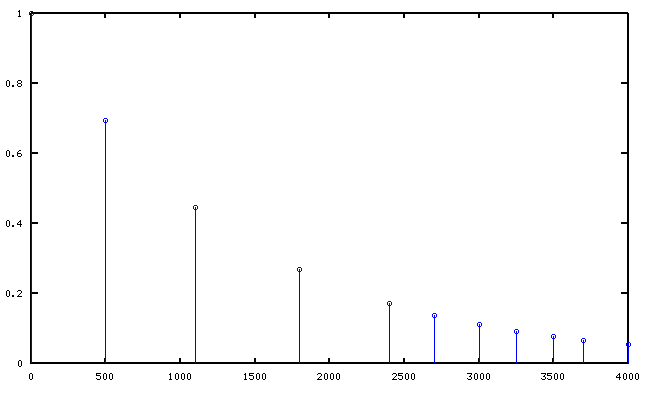
\includegraphics[scale=0.5]{Bilder/signalabgriffe.png}
	\caption{Raumimpulsantwort}
	\label{labelname}
\end{figure}
Da wir mit einem Ringspeicher arbeiten, sind die Indizes der Abgriffe zwar konstant, jedoch relativ zum Index des neuen Wertes. Auch hier wurde mit einer AND-Operation mit 0x0fff gearbeitet, damit der index bis maximal 4095 geht und dann von 0 fortgesetzt wird.
Zur Berechnung der Koeffizienten wurde eine Exponentialfunktion zur Basis e folgender Form gewählt:

$k=exp(-3/4096*i)$
 
wobei i der Index des Abgriffes und k der resultierende Koeffizient ist.
Beim Multiplizieren eines Abgriffes mit einem Koeffizienten wird außerdem das Ergniss durch 4 geteilt um eine Übersteuerung zu vermeiden. Realisiert wurde das durch ein 2-fachen Right-Shift.
Am ende des Prozesses wird der Akkumulator an den Ausgang übergeben, welcher weiter an den DA-Wandler gegeben wird. Dabei ist darauf zu achten den Akkumulator durch ein 16-fachen Right-Shift für ein fractional-16 Format zu konvertieren.
Der Akkumulator wird ebenfalls beim nächsten Aufruf des Prozess mit dem Faktor 0.25, also zweimaligem Right-Shift auf den nächsten neuen Wert addiert, um die Rückkopplung zu realisiern.
Weiterhin ist darauf zu achten das die Opperation des Akkumulierens nicht stattfinden kann, wenn der Buffer noch nicht komplett gefüllt ist. Es wurde eine Load-Variable deklariert welche mit jedem Prozessaufruf inkrementiert wird. Bei jedem Prozessdurchlauf wird getestet ob diese den Wert 4095 übersteigt, wenn ja wird sie nicht weiter inkrementiert und die Akkumulation wird vorgenommen.

%%%%%%%%%Quellcode%%%%%%%%%%%%%%%%%%%%%%%%%%%%%%%%%%%%%%%%%%%%%%%%%%%%%%%%%%%%
\subsection{Quellcode}
An dieser Stelle sei ein Kurzer Einblick in die wesentlichen Teiles des Quellcodes unseres Projektes geboten.
 \\
\newline
Ein Array mit Koeffizienten zur Berechnung der internen Filterstruktur wird bereits in der Datei Main.c deklariert und definiert.
\newline%

\lstset{% general command to set parameter(s)
language=C,%Spache angeben
numbers=left,%Zeilennummern anzeigen
breaklines=true, % Zeilen werden Umgebrochen
keywordstyle=\color{magenta}\bfseries,%keywords hervorheben
commentstyle=\color{blue},
identifierstyle=\color{cyan},
stringstyle =\itshape\color{red}
}
\begin{lstlisting}[title=Koeffizientenarray Dekleration \& Definition in Main.c]
fract16 fKof[11]={0.99999r16,0.693r16,0.447r16,0.268r16,0.172r16,0.138r16,0.111r16,0.093r16,0.077r16,0.066r16,0.053r16};//Koeffizienten Array 
\end{lstlisting}

\newpage
In der Datei Main.c findet sich auch, wie in jedem C-Programm, die main Funktion.

\lstset{% general command to set parameter(s)
language=C,%Spache angeben
%[title=main-Funktion in Main.c]
numbers=left,%Zeilennummern anzeigen
breaklines=true, % Zeilen werden Umgebrochen
keywordstyle=\color{magenta}\bfseries,%keywords hervorheben
commentstyle=\color{blue},
identifierstyle=\color{cyan},
stringstyle =\itshape\color{red}
}
\begin{lstlisting}
void main(void)
\end{lstlisting}
Sie beschreibt den we
sentlichen Programmablauf. Es wird hier zunächst überprüft, ob neue Werte am Analog-Digital-Wandler (ADC) anliegen. Anschließend wird der Programm Modus ausgewählt. Dies bestimmt, wie anliegende Werte ggf. bearbeitet werden. Hierbei sind vier verschiedene Prozesse auswählbar.

%\newpage

\lstset{% general command to set parameter(s)
language=C,%Spache angeben
%title=Endlosschleife in Main.c,%Titel setzten
numbers=left,%Zeilennummern anzeigen
breaklines=true, % Zeilen werden Umgebrochen
keywordstyle=\color{magenta}\bfseries,%keywords hervorheben
commentstyle=\color{blue},
identifierstyle=\color{cyan},
stringstyle =\itshape\color{red}
}
\begin{lstlisting}[title=Endlosschleife in Main.c]
   while(1)
   { //--------------------------------------------------------
     if(NewAdcData != 0)                // if new data from ADC
      { //-----------------------------------------------------
        NewAdcData = 0;                 // set flag back   
        //-------------------------------------------------
        //  Choose Type of Signal processing                 
        //-------------------------------------------------
        switch(PrMode) 
         {
           case 0: Process_A();break;   // Signal-Process-A
           case 1: Process_B();break;   // Signal-Process-B
           case 2: Process_C();break;   // Signal-Process-C
           case 3: Process_D();break;   // Signal-Process-D
          }
        //-------------------------------------------------
      } // end if NewAdcData
     //----------------------------------------------------
     if(NewTimerEvent != 0)             // if new TimerEvent
      { //-------------------------------------------------
        NewTimerEvent = 0;              // set flag back    
        //-------------------------------------------------
        Process_Tim0();
        //-------------------------------------------------
      }  // end if NewTimerEvent
        //-------------------------------------------------
   }  // end endless while-loop
\end{lstlisting}%
.
\\

Die Signalverarbeitung, welche den künstlichen Hall implementiert, wird im Prozess A durchgeführt. Die Prozesse B und C schleifen lediglich die Eingänge des Signalprozessors auf dessen Ausgänge durch. Diese Modi dienen der besseren Veranschaulichung bei Live-Demos.  Der Unterschied zwischen beiden Prozessen besteht darin, dass Prozess B das Signal mit einem Faktor 0,5 multipliziert und Prozess C keine interne Bearbeitung vornimmt. Legt man gemäß dem genannten Versuchsaufbau ein Audiosignal an den Eingang des Signalprozessors, so ist dieses Signal unter Nutzung des Prozess\_Modus C am Ausgang direkt zu hören. Verwendet man den Prozess\_Modus B ist das Eingangssignal am Ausgang lediglich etwas leiser zu hören. Prozess D ist nicht implementiert.

\newpage

\lstset{% general command to set parameter(s)
language=C,%Spache angeben
%title=Endlosschleife in Main.c,%Titel setzten
numbers=left,%Zeilennummern anzeigen
breaklines=true, % Zeilen werden Umgebrochen
keywordstyle=\color{magenta}\bfseries,%keywords hervorheben
commentstyle=\color{blue},
identifierstyle=\color{cyan},
stringstyle =\itshape\color{red}
}
\begin{lstlisting}[title=PROCESS\_A aus Processing.c]
//--------------------------------------------------
// Function:    PROCESS_A for Signal-Processing
//--------------------------------------------------
void Process_A(void)               
 { //------------------------
 	fIn    =   fInp_1;          // neuen Wert speichern
	
	ip=ip&0x00000fff;			// Kreisindizierung mit 4096 indizes
	fBuf[ip]=fIn<<15;			// 16 bit in 32 bit fract also 16 mal nach links schieben
	    // und multiplizieren mit Faktor 0.5, also 1 mal nach rechts schieben
	
	fBuf[ip]+=fAcc>>2;	//Rueckkoplung mit Faktor 0.25
	int k=0;		// Koeffizienten-Index

	if(ic>4095){                // wenn Buffer gefuellt ist (buffer load > 4095
		fAcc=0;
		
		fTmp_16=fKof[0];            // Koeffizient laden
		k=ip;                       // Bufferindex relativ zum letzten Wert (hier 0)
		k=k&0x00000fff;             // Kreisindizierung des buffers, max 4095
		fTmp2_16=fBuf[k]>>16;       // fract32 Buffer-Wert in fract16 Variable
		fTmp2_32=fTmp2_16*fTmp_16;  // 16 bit Multiplikation mit 32 bit Ergebniss
		
		fTmp2_32>>1;                /* Ergebnis muesste 1 mal links geschoben werden damit das fract32 format stimmt, aber multiplikation mit Faktor 0.25 (2mal rechts schieben) ergibt 1 mal rechts schieben
		                             */
		                             
		fAcc+=fTmp2_32;             // Ergebnis akkumulieren

		
		
		fTmp_16=fKof[1];
		k=ip+500;               // Bufferindex relativ zum letzten Wert (hier 500)
		k=k&0x00000fff;
		fTmp2_16=fBuf[k]>>16;
		fTmp2_32=fTmp2_16*fTmp_16;
		fTmp2_32>>1;
		fAcc+=fTmp2_32;
		
		fTmp_16=fKof[2];
		k=ip+1100;
		k=k&0x00000fff;
		fTmp2_16=fBuf[k]>>16;
		fTmp2_32=fTmp2_16*fTmp_16;
		fTmp2_32>>1;
		fAcc+=fTmp2_32;

		fTmp_16=fKof[3];
		k=ip+1800;
		k=k&0x00000fff;
		fTmp2_16=fBuf[k]>>16;
		fTmp2_32=fTmp2_16*fTmp_16;
		fTmp2_32>>1;
		fAcc+=fTmp2_32;
		
		fTmp_16=fKof[4];
		k=ip+2400;
		k=k&0x00000fff;
		fTmp2_16=fBuf[k]>>16;
		fTmp2_32=fTmp2_16*fTmp_16;
		fTmp2_32>>1;
		fAcc+=fTmp2_32;
		
		fTmp_16=fKof[5];
		k=ip+2700;
		k=k&0x00000fff;
		fTmp2_16=fBuf[k]>>16;
		fTmp2_32=fTmp2_16*fTmp_16;
		fTmp2_32>>1;
		fAcc+=fTmp2_32;
		
		fTmp_16=fKof[6];
		k=ip+3000;
		k=k&0x00000fff;
		fTmp2_16=fBuf[k]>>16;
		fTmp2_32=fTmp2_16*fTmp_16;
		fTmp2_32>>1;
		fAcc+=fTmp2_32;
		
		fTmp_16=fKof[7];
		k=ip+3250;
		k=k&0x00000fff;
		fTmp2_16=fBuf[k]>>16;
		fTmp2_32=fTmp2_16*fTmp_16;
		fTmp2_32>>1;
		fAcc+=fTmp2_32;
		
		fTmp_16=fKof[8];
		k=ip+3500;
		k=k&0x00000fff;
		fTmp2_16=fBuf[k]>>16;
		fTmp2_32=fTmp2_16*fTmp_16;
		fTmp2_32>>1;
		fAcc+=fTmp2_32;
		
		fTmp_16=fKof[9];
		k=ip+3700;
		k=k&0x00000fff;
		fTmp2_16=fBuf[k]>>16;
		fTmp2_32=fTmp2_16*fTmp_16;
		fTmp2_32>>1;
		fAcc+=fTmp2_32;
		
		fTmp_16=fKof[10];
		k=ip+4000;
		k=k&0x00000fff;
		fTmp2_16=fBuf[k]>>16;
		fTmp2_32=fTmp2_16*fTmp_16;
		fTmp2_32>>1;
		fAcc+=fTmp2_32;
	}
   
	if(ic<4096){			// ic max 4095
        ic++;			    // Buffer load erhoehen, falls nicht schon voll
    }
    ip++;                   // pointer auf ringbuffer erhoehen (kreisindizierung)
	
    fOut_1=fAcc>>16;	    // Akkumulator Wert auf beide Ausgaenge legen
                            // 16 mal rechtsschieben, da fract32 zu fract16 konvertierung
	fOut_2=fOut_1;
   
    PutDAC(DAC_1R, fOut_1); // Write DAC 1R
    PutDAC(DAC_1L, fOut_2); // Write DAC 1L
   //------------------------
 }
\end{lstlisting}

\section{Schluss}
Das Projekt "`Künstlicher Hall"' ist eine gelungene Zusammenfassung der Lerninhalte aus dem Modul Signalprozessortechnik.
Durch die Arbeit am Projekt ist es uns gelungen das Verständnis für die Feinheiten digitaler Signalverarbeitung mit Signalprozessoren zu vertiefen. Es galt die Schwerpunkte der Digitalen Signalverarbeitung, insbesondere im Bereich der digitalen Filter, mit den Finessen und Echtzeitproblematiken von Signalprozessoren unter einen Hut zu bringen. Dies ist uns im vorgestellten Projekt meiner Meinung nach erfolgreich geglückt.

Das Vorgegebene Framework war hierzu eine sehr große Stütze. Es erlaubte es uns, unsere Konzentration ganz auf den Schwerpunkt der Hall-Erzeugung zu legen. Die Auseinandersetzung mit dem Thema Hall führe zudem zu noch besserem Verständnis für die digitalen Filterstrukturen FIR \& IIR.
\\

Am Ende des Projektes bleibt nun noch die Präsentation für die anderen Teilnehmer des Moduls Signalprozessortechnik. Wir hoffen diese mit unserem Projekt begeistern zu können.
\\

Natürlich bietet solch ein Projekt stets enormes Potential die Arbeit daran noch viel länger fortzusetzen. Denkbar wären u.a. verschiedene Hall-Effekte. So könnte man Hall Implementieren, welcher stark an Hall erinnert, den man aus kleinen Badewannen-Zimmern kennt, oder gar Hall wie er in großen Kirchenräumen zu finden ist. Durch Variation der Anzahl an Zurückgeführter Koeffizienten und natürlich auch Variation der Koeffizienten selbst eröffnet sich hierbei ein enormer Bereich an denkbaren Möglichkeiten und Erweiterungen.

Besonders im Bezug auf Signalprozessoren bietet sich natürlich die Möglichkeit den geschriebenen Code zu Optimieren. Schleifen, If-Anweisungen und Funktionsaufrufe könnten im Assembler-Sprache programmiert und effizienz-technisch optimiert werden.
Hier bietet sich noch viel Potential die Echtzeitfähigkeit des Systems zu steigern und die benötigte Zeit zur Signalverarbeitung zu reduzieren.
Aus Zeitlichen Gründen sind wir jedoch leider dazu nicht mehr in der Lage gewesen. So haben wir uns auf die Funktionalität eines ersten, präsentierfähigen Halls beschränkt und freuen uns schon auf die Präsentation der Projekte vor allen Modulteilnehmern.

%Beginn einer neuen Seite
\clearpage

\section{Literaturverzeichnis}
\vspace{1.5cm}
 %Eine einfache Liste
 \begin{itemize} 
\item lsf.uni-rostock.de, Veranstaltungsnummer 24141, Vorlesung Signalprozessortechnik, SS 2012
\item Vorlesungsskript Signalprozessortechnik, SS2012
\item Versuchsanleitung Nr. 2 "`Digitale Filter"', Praktikum zur Veranstaltung "`Digitale Signalverarbeitung"' Institut für Nachrichtentechnik, Universität Rostock
\end{itemize}





\end{document}
%-------------------
%Hier endet der Text deiner Hausarbeit
%-------------------
%
%
%
%Ein längeres Zitat
%\begin{quote}
%Vel eum iriure dolor in hendrerit in vulputate velit esse. Modo typi qui nunc nobis, videntur %sollemnes in\footnote{fußnoten text}.
%\end{quote}